
\documentclass[12pt]{article}
\usepackage{fullpage,amsmath,amssymb,graphicx}

\usepackage{setspace}
\spacing{1}

\usepackage{textpos}
\usepackage{tikz}
\usepackage{pgf}
\usepackage{amssymb}
\usepackage{enumerate}
\usepackage{xcolor}
\usepackage{graphicx}
\usepackage{subcaption}
\usepackage{tabularx}
\usepackage{colortbl}
\usepackage{multicol}
\usepackage{longtable}
\usepackage{hyperref}
\usepackage{comment}
\usepackage{listings}



\definecolor{encabezado}{rgb}{0.74, 0.83, 0.9}

\begin{document}

\hfill\\
\rule{\textwidth}{1.5pt}

\begin{minipage}[t]{85mm}
  \begin{tabular}{l}
    \textbf{\large Instituto Tecnológico de Costa Rica} \\  
    \textbf{Escuela de Ingeniería Electrónica} \\
    \textbf{Trabajo Final de Graduación} \\
    \textbf{Proyecto:} Método basado en aprendizaje reforzado \\para el control automático de una planta no lineal. \\
    \textbf{Estudiante:} Oscar Andrés Rojas Fonseca \hspace{3cm}\rule{4.5cm}{1.5pt}\\
    I Semestre 2024 \hspace{8.5cm}\textbf{Firma del asesor}
  \end{tabular}
\end{minipage}
\hfill\\
\rule{\textwidth}{1.5pt}


\section*{Bitácora de trabajo}

%\begin{table}[h]
\begin{minipage}[h]{\textwidth}
	\centering
	\begin{tabularx}{\textwidth}{|p{2cm}|X|X|p{2cm}|} 
		\hline
		\rowcolor{encabezado}
		\textbf{Fecha} & 
		\textbf{Actividad} & 
		\textbf{Anotaciones} & 
		\textbf{Horas dedicadas} \\ \hline
		% ***************************************************************
	 	08/04/2024 & 
	 	$\mathbf{1}.$ Prueba de adaptación del código $CartPoleDQN.ipynb$ para manejo de variables continuas. & 
	 	$a)$ Se buscaron opciones para la sustitución de la función $torch.gather()$ utilizada en el código original. \newline & 
	 	4 horas \\
		% ***************************************************************
		09/04/2024 & 
	 	$\mathbf{2}.$ Pruebas de implementación $CUDA$ en Windows. &
	 	$a)$ Reinstalación de paquetería $CUDA\,\, 12.1$ y librería $PyTorch\,\, 2.2.2$. \newline
	 	$b)$ La implementación $CUDA$ fue exitosa, reduciendo importantemente los tiempos de entrenamiento. \newline & 
	 	4 horas \\
	 	% ***************************************************************
		09/04/2024 & 
	 	$\mathbf{3}.$ Pruebas de entrenamiento del modelo $Pendulum\, DQN$. &
	 	$a)$ Se implementó una primera versión de la adaptación del código original para el manejo de variables continuas. \newline
	 	$b)$ Entrenamiento de modelo controlador de hasta $600$ episodios. \newline & 
	 	4 horas \\
	 	% ***************************************************************
	 	10/04/2024 & 
	 	$\mathbf{4}.$ Reunión de seguimiento con el asesor del proyecto. & 
	 	$a)$ Revisión de avance en el código y errores de forma.  \newline
	 	$b)$ Se acordó realizar entrenamientos con diferentes formatos de indicación del $target\_angle$.  \newline & 
	 	2 horas \\
	 	\hline
	\end{tabularx}
\end{minipage}	 	
	 	
	 	% ***************************************************************
\hfill\\
\begin{minipage}[h]{\textwidth}
	\centering
	\begin{tabularx}{\textwidth}{|p{2cm}|X|X|p{2cm}|} 
		\hline		
		
	 	% ***************************************************************
	 	11/04/2024 & 
	 	$\mathbf{5}.$ Corrección de potenciales errores en el código $PendulumDQN$ señalados por asesor. &
	 	$a)$ Replanteo de función de recompensa $calculate\_ reward()$ para evitar salto. \newline
	 	$b)$ Adición de lógica para guardado de $checkpoints$ al entrenamiento y corrección del guardado del modelo. \newline & 
	 	8 horas \\
	 	% ***************************************************************
	 	12/04/2024 & 
	 	$\mathbf{6}.$ Continuación de corrección de errores potenciales en el código. &
	 	$a)$ Replanteo de función $select\_ action()$; cambio de acción aleatoria en exploración a adición de ruido a la opción elegida. \newline & 
	 	4 horas \\
	 	% ***************************************************************
	 	12/04/2024 & 
	 	$\mathbf{7}.$ Estudio de conceptos $MDP$ \cite{PAlvaradoMDP1} y $DQN$ \cite{PAlvaradoDQN1} . &
	 	$a)$ Revisión de aplicación mediante $MDP$ dada la mensión en una fuente en línea donde se utiliza \cite{CartPoleRLcrtl1}. \newline
	 	$b)$ Estudio de teoría $DQN$ para mejor comprensión de la lógica de la función $optimize\_ model()$ del código original \cite{DQNCart} y su adaptación a $Pendulum$. \newline & 
	 	4 horas \\
	 	% ***************************************************************
	 	12/04/2024 & 
	 	$\mathbf{8}.$ Pruebas de entrenamiento de modelos $CartPole$ y $Pendulum$. &
	 	$a)$ Se crearon los cuadernos $ctrlCartPoleDQN.ipynb$ y $ctrlPendulumDQN.ipynb$ para pruebas de carga de modelos. \newline
	 	$b)$ Entrenamiento del modelo $Pendulum\_1000eps.pth$. \newline
	 	$c)$ Se descubrió un error grave en $select\_action()$, corrección en proceso. \newline & 
	 	6 horas \\
	 	% ***************************************************************
	 	
	 	\hline
		\multicolumn{3}{|r|}{Total de horas de trabajo:} & 36 horas \\ 
	 	\hline                 
	\end{tabularx}
\end{minipage}
%\end{table}



% *****************************************************************************
% *****************************************************************************
% *****************************************************************************

\section*{Contenidos de actividades}

\subsection*{Primeros entrenamientos con $PendulumDQN$}

La primera versión de la adaptación del código a variable continua permitió los primeros entrenamientos del modelo controlador de $Pendulum$, donde la implementación del procesamiento con $CUDA$ permitió la disminución del tiempo de entrenamiento a aproximadamente a la mitad del tiempo de procesamiento con $CPU$, permitiendo los entrenamientos de hasta $600$ episodios en $20$ minutos y posteriores $1000$ episodios en aproximadamente $40$ minutos.

Los modelos anteriormente mencionados, a pesar de las comparaciones con el modelo exitoso entrenado de $CartPole$ a $600$ episodios, no presenta mejoría en las pruebas realizadas, por lo que se procede a plantear una nueva forma de la adaptación al manejo de valores continuos en la función $optimize\_ model()$.

\subsection*{Estudio de $MDP$ y $DQN$}

Se requirió una revisión de la teoría que sustenta al método $DQN$ en \cite{PAlvaradoDQN1} para comprender a mayor profundidad el proceso que realiza la función $optimize\_model()$, de manera que la base de la técnica de $Q-learning$ también fue estudiada.

Además, la presencia del proceso de decisión de Markov ($MDP$) en algunas de las revisiones de las opciones de implementación de variable continua al método $DQN$ \cite{CartPoleRLcrtl1}, requirió un análisis respectico del algoritmo, por lo que se estudió en \cite{PAlvaradoMDP1}, también a manera de contextualización al tema del $Q-learning$.



%\begin{figure}[h]
%	\centering
%	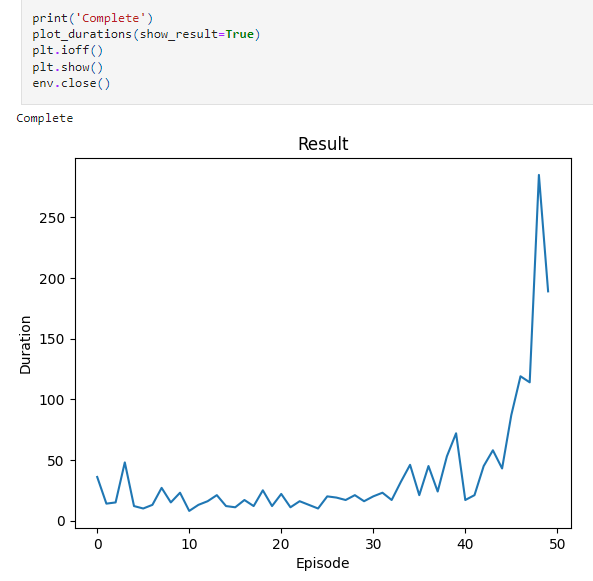
\includegraphics[scale=0.6]{Fig/CapturaCartPole1.png}
%	\caption{Resultado de entrenamiento del modelo para $CartPole$ con $50$ episodios.}
%	\label{fig:Cart1}
%\end{figure}	

\newpage

\section*{Referencias}
\renewcommand\refname{}
\bibliographystyle{IEEEtran}
\bibliography{references}





\end{document}
